\documentclass[11pt]{article}

% =========================
% Packages
% =========================
\usepackage[margin=1in]{geometry}
\usepackage{amsmath, amssymb, amsfonts}
\usepackage{booktabs}
\usepackage{array}
\usepackage{enumitem}
\usepackage{hyperref}
\usepackage{xcolor}
\usepackage{graphicx}
\usepackage{tikz}
\usepackage{longtable}
\usepackage{multirow}
\usepackage{caption}
\usepackage{float}
\usepackage{pdflscape}
\usepackage{listings}

\usetikzlibrary{arrows.meta, positioning, shapes.geometric, shapes.misc, fit, backgrounds}

% =========================
% Styling
% =========================
\hypersetup{
    colorlinks=true,
    linkcolor=blue,
    urlcolor=blue,
    citecolor=blue
}

\setlist[itemize]{leftmargin=*, topsep=3pt, itemsep=2pt}
\setlist[enumerate]{leftmargin=*, topsep=3pt, itemsep=2pt}
\setlength{\parindent}{0pt}
\setlength{\parskip}{6pt}

\lstset{
    basicstyle=\ttfamily\small,
    breaklines=true,
    frame=single,
    columns=fullflexible
}

\newcommand{\todo}[1]{\textcolor{red}{\textbf{TODO:} #1}}
\newcommand{\decision}[1]{\textcolor{blue}{\textbf{Decision:} #1}}
\newcommand{\risk}[1]{\textcolor{red}{\textbf{Risk:} #1}}
\newcommand{\note}[1]{\textcolor{teal}{\textbf{Note:} #1}}

% =========================
% Title
% =========================
\title{\textbf{Team Review Report: Parallel Implementation Plan for Random Projections and Low-Rank Structure in Financial Return Data}}
\author{Vishal Jha, Adel Sahuc \\ NYU MS Computer Science}
\date{}

\begin{document}
\maketitle

\vspace{-1.0em}

\begin{center}
\textbf{Primary Paper:} Michael B. Cohen, Thathachar S. Jayram, and Jelani Nelson. \\
\emph{Simple Analyses of the Sparse Johnson--Lindenstrauss Transform.} SOSA 2018.
\end{center}

\tableofcontents
\newpage

% ============================================================
\section{Executive Summary}

This document defines the proposed implementation plan for our project on random projections for cross-sectional compression of financial asset return data. The project is motivated by the SOSA 2018 paper \emph{Simple Analyses of the Sparse Johnson--Lindenstrauss Transform} by Cohen, Jayram, and Nelson. That paper studies sparse Johnson--Lindenstrauss transforms, which are randomized linear maps that preserve Euclidean geometry while using substantially fewer nonzero entries than dense random projections.

Our project asks whether this sparse, data-independent compression perspective remains useful in a structured financial setting. Financial asset returns are not arbitrary high-dimensional vectors. They are strongly correlated, affected by common market and sector forces, and often approximately governed by a small number of latent factors. This suggests that financial return matrices may have approximate low-rank structure. PCA or truncated SVD should exploit this structure directly, while sparse JL and dense Gaussian random projections are oblivious to it.

The central research question is:

\begin{quote}
\textbf{When does data-independent sparse JL compression preserve the geometry of factor-structured financial return data, and when does data-adaptive PCA dominate?}
\end{quote}

The proposed empirical study compares four representations:

\begin{enumerate}
    \item Raw uncompressed return vectors.
    \item Dense Gaussian Johnson--Lindenstrauss projections.
    \item Sparse Johnson--Lindenstrauss projections.
    \item PCA / truncated SVD.
\end{enumerate}

The primary real-data experiment uses a cross-sectional equity return matrix built from S\&P 500 constituents (today's membership, $\sim$500 tickers), sourced from a pinned public Kaggle dataset for reproducibility. Each row is one trading day and each column is one asset; each row is treated as a market-state vector. The project evaluates whether compressed representations preserve distances, nearest neighbors, clustering structure, and unusual market days.

The secondary controlled experiment uses synthetic factor-model data of the form
\[
X = F B^\top + E,
\]
where $F$ contains latent factor returns, $B$ contains asset factor loadings, and $E$ is idiosyncratic noise. This synthetic experiment is critical because it lets us directly vary the true factor rank and noise level, allowing us to isolate when PCA should beat JL and when sparse JL may remain competitive.

This updated plan adds two major implementation improvements:

\begin{enumerate}
    \item \textbf{Parallel execution plan:} The experiment grid is large enough that a purely linear implementation may be slow. We therefore design the system so that experiment configurations can run independently using a backend abstraction. The preferred backend is Ray when available, with a local sequential fallback for reproducibility.

    \item \textbf{Expanded figure plan:} The final report should not rely on only a few aggregate plots. The implementation must generate at least 40 figures covering raw data diagnostics, PCA structure, JL grid-search behavior, real-data metrics, COVID-specific diagnostics, synthetic factor-model experiments, runtime/memory tradeoffs, and robustness checks.
\end{enumerate}

% ============================================================
\section{Final Configuration for Team Review}

The following configuration is the proposed default. Once approved, this should be frozen and converted into an implementation plan for the coding agent.

\begin{table}[H]
\centering
\caption{Proposed Experimental Configuration}
\begin{tabular}{p{0.34\linewidth} p{0.56\linewidth}}
\toprule
\textbf{Component} & \textbf{Decision} \\
\midrule
Asset universe & S\&P 500 today's constituents ($\sim$500 names); survivorship-biased, declared in limitations \\
Data source & Kaggle: \texttt{andrewmvd/sp-500-stocks} (Larxel), pinned dataset version; yfinance fallback if unavailable \\
Selection framework & Three-layer pipeline: (1) S\&P 500 candidate pool, (2) rank by avg dollar volume, (3) elimination pipeline (data integrity + anomaly filters), then take \texttt{top\_100}, \texttt{top\_200}, or \texttt{all\_survivors} \\
Date range & 2014-01-01 to 2024-12-31 \\
Return type & Daily log returns \\
Data matrix & Rows = trading days, columns = assets \\
Missing data policy & No imputation in the primary experiment; tickers with missing values are dropped at Stage 1 of the elimination pipeline; no reserve replacement \\
Preprocessing & Z-score each asset using training-set statistics only \\
Train/test split & Chronological 70/30 split for primary evaluation \\
Core methods & Raw, dense Gaussian JL, sparse JL, PCA / truncated SVD \\
Primary target dimensions & $k \in \{5, 10, 20, 30, 50, 100\}$ \\
Sparse JL sparsity & Primary grid $s \in \{1, 3, 5\}$; primary value $s=3$ \\
Random seeds & 10 seeds for randomized JL methods \\
Real-data metrics & Distance distortion, nearest-neighbor overlap, clustering ARI, anomaly recall, runtime, memory \\
COVID-specific evaluation & Full sample including COVID, full sample excluding COVID, COVID-stress-only window \\
Synthetic model & $X = F B^\top + E$ \\
Synthetic ranks & $r \in \{3, 5, 10, 20\}$ \\
Synthetic noise levels & $\sigma \in \{0.1, 0.5, 1.0\}$ \\
Parallel execution & Ray backend preferred for grid experiments; local backend required as fallback \\
Minimum figure count & At least 40 generated figures \\
Primary story & PCA dominates under strong low-rank structure; sparse JL becomes competitive when structure weakens, noise increases, $k$ increases, or efficiency matters \\
\bottomrule
\end{tabular}
\end{table}

% ============================================================
\section{Research Framing}

\subsection{Primary Paper Context}

The primary paper, \emph{Simple Analyses of the Sparse Johnson--Lindenstrauss Transform}, studies sparse variants of the Johnson--Lindenstrauss transform. The classical Johnson--Lindenstrauss lemma says that a set of high-dimensional points can be embedded into a much lower-dimensional Euclidean space while approximately preserving pairwise distances. Dense Gaussian random projections are a common way to achieve this, but dense projections can be computationally expensive when the original dimension is large.

Sparse JL transforms aim to preserve the same basic geometric behavior while reducing computational cost. Instead of multiplying by a dense random matrix, the input is multiplied by a sparse random matrix with relatively few nonzero entries. The SOSA paper is important because it provides simple analyses of these sparse transforms and helps explain why sparse random projections can retain useful distance-preservation guarantees.

\subsection{Why Financial Return Data Is a Meaningful Testbed}

Financial return data is a structured domain. Cross-sectional equity returns are affected by common forces such as:

\begin{itemize}
    \item market-wide movements,
    \item sector-level effects,
    \item style factors,
    \item macroeconomic shocks,
    \item liquidity and volatility regimes.
\end{itemize}

This means the data may lie close to a low-dimensional factor space. A simplified factor model has the form
\[
x_t = B f_t + \epsilon_t,
\]
where $x_t \in \mathbb{R}^N$ is the return vector across $N$ assets at time $t$, $B \in \mathbb{R}^{N \times r}$ contains factor loadings, $f_t \in \mathbb{R}^r$ contains factor returns, and $\epsilon_t$ is idiosyncratic noise.

This creates a natural tension:

\begin{itemize}
    \item PCA is data-adaptive and should exploit low-rank factor structure.
    \item Sparse JL is data-independent and does not explicitly learn the factor space.
    \item Dense Gaussian JL is also data-independent but less sparse and more computationally expensive.
\end{itemize}

The project therefore tests whether sparse JL remains empirically useful when the data has financial structure that PCA is designed to exploit.

\subsection{Core Research Questions}

The implementation should directly support the following three research questions:

\begin{enumerate}
    \item \textbf{Generalization of sparse JL intuition:} To what extent do the structure-preservation properties of sparse JL transforms remain meaningful when applied to highly correlated financial asset return data rather than generic high-dimensional vectors?

    \item \textbf{Low-rank factor structure vs. sparse JL:} When asset returns lie near an approximate low-rank factor model, when do sparse random projections preserve market geometry nearly as well as PCA, and when does the low-rank structure make PCA fundamentally superior at the same compressed dimension?

    \item \textbf{Role of market structure:} Which properties of financial data, such as factor strength, cross-sectional correlation, volatility regime, and COVID-style stress periods, most strongly affect whether sparse JL projections preserve nearest neighbors, clustering structure, and unusual market states?
\end{enumerate}

% ============================================================
\section{Data Design}

\subsection{Real Financial Dataset}

The real dataset consists of daily adjusted close prices for U.S. equities in the S\&P 500. The team adopts the following data plan:

\textbf{Asset universe:} S\&P 500 constituents (current membership, $\sim$500 names). The full S\&P 500 is preferred over the smaller S\&P 100 because (a) it provides a higher-dimensional cross-section ($N \approx 500$), making the compression research question more interesting, and (b) historical S\&P 500 data is far better supported by public sources than S\&P 100 data.

\textbf{Survivorship bias acknowledgement:} Using today's S\&P 500 backfilled to 2014 is survivorship-biased. Constituents that were in the S\&P 500 in 2014 but were later acquired, bankrupt, or demoted (e.g., Time Warner, Sprint, Allergan) are excluded. This is a known limitation. The project's research question concerns compression geometry on real structured financial data, not trading-strategy realism, so this bias is acceptable as long as it is clearly stated. Survivorship bias is addressed in the limitations section of the final report (see Section~\ref{sec:risks}).

\subsection{Data Source}\label{sec:data-source}

\textbf{Primary source:} Kaggle dataset \emph{S\&P 500 stocks (daily updated)} maintained by user \texttt{andrewmvd} (Larxel). Available at:
\begin{quote}
\url{https://www.kaggle.com/datasets/andrewmvd/sp-500-stocks}
\end{quote}

The implementation must:

\begin{enumerate}
    \item Pin a specific dataset version (record the Kaggle version number and download date in \texttt{configs/experiment\_config.yaml}).
    \item Commit the downloaded CSV files to \texttt{data/raw/} so the project is reproducible without re-downloading.
    \item Validate the CSV against the no-imputation policy in Section~\ref{sec:missing-data}.
\end{enumerate}

\textbf{Why a public CSV instead of a live API:} Live APIs (yfinance, Tiingo, Alpha Vantage) introduce reproducibility risk because returned values depend on download timing, vendor adjustment choices, and API stability. A pinned Kaggle CSV gives a frozen, version-controlled input that any reviewer can re-run and obtain identical results.

\textbf{Why Kaggle is acceptable for a research project:} The S\&P 500 historical price dataset is heavily used by the academic and student community. It is not the canonical source (CRSP via WRDS is), but for a research project on compression geometry it is a defensible trade-off given the lack of free WRDS access. The bias and quality trade-offs are documented in Section~\ref{sec:risks}.

\textbf{Fallback source:} If the Kaggle dataset becomes unavailable or fails validation, the data pipeline must support a yfinance-based fallback that reproduces the same schema. The fallback uses the same fixed ticker list (today's S\&P 500), scraped from Wikipedia's \emph{List of S\&P 500 companies} page.

\textbf{Validation cross-check (recommended):} For a small random sample of tickers (e.g., 5--10 names), the pipeline should compare Kaggle adjusted-close values against a second source (yfinance or Stooq) for a handful of dates. Material disagreements should be logged. This is a sanity check, not a full audit.

\subsection{Stock Selection Rules}\label{sec:selection-rules}

The pipeline applies a deterministic three-layer framework to convert the S\&P 500 candidate pool into a final analysis universe. The three layers separate \emph{candidate sourcing} from \emph{ranking} from \emph{elimination}, so each can be reasoned about independently.

\subsubsection{Layer 1: Candidate Pool}

The candidate pool is today's S\&P 500 constituents ($\sim$500 names, with $\sim$503 actual rows due to dual-class shares such as GOOG/GOOGL). The list is loaded from the pinned Kaggle dataset's ticker manifest. Output: \texttt{data/processed/candidate\_universe.csv}.

\subsubsection{Layer 2: Ranking Metric}

Tickers in the candidate pool are ranked by \textbf{average daily dollar volume} over the full study window:
\[
\text{Rank}_i =
\frac{1}{T}
\sum_{t=1}^{T}
P_{t,i} \cdot V_{t,i},
\]
where $P_{t,i}$ is the adjusted close price and $V_{t,i}$ is the daily share volume.

This metric was chosen because:
\begin{itemize}
    \item It composes naturally with the elimination rules: stocks that delisted mid-period get zero volume after delisting and rank low automatically.
    \item It is a better proxy for ``stocks that traded actively and reliably'' than market capitalization, which is dominated by a handful of mega-caps.
    \item Both inputs ($P$ and $V$) are available in any standard data source, including the Kaggle CSV.
\end{itemize}

The ranking is computed once over the full window and frozen. Output: \texttt{data/processed/ranked\_universe.csv}.

\subsubsection{Layer 3: Elimination Pipeline}

The following filters are applied in order. Each filter logs the number of tickers it drops and the list of dropped ticker symbols.

\textbf{Stage 1 -- Data integrity filter.} Drop a ticker if any of the following hold:
\begin{itemize}
    \item Any NaN in adjusted close inside $[2014\text{-}01\text{-}01, 2024\text{-}12\text{-}31]$.
    \item The ticker was delisted before 2024-12-31 (last trade date earlier than the window end). This is the bankrupt / acquired / removed-from-index case.
    \item Fewer than 95\% of expected trading days are present.
    \item Any single-day return $|r| > 0.5$ that does not correspond to a known corporate action (treated as a data error).
\end{itemize}

\textbf{Stage 2 -- Anomaly filter.} Drop a ticker if any of the following hold:
\begin{itemize}
    \item More than $N_{\text{flat}}$ consecutive days of exactly zero return (likely halted or stale data); recommended $N_{\text{flat}} = 10$.
    \item Adjusted close exactly constant for more than 5 consecutive days (likely a data error).
\end{itemize}

\note{No liquidity floor is applied. The ranking metric already pushes illiquid names down the list, and an explicit dollar-volume threshold would impose an arbitrary cutoff without scientific justification for a compression-geometry study.}

\textbf{Stage 3 -- Selection.} From the surviving tickers, take the top-$N$ by the ranking metric. Supported choices:
\begin{itemize}
    \item \texttt{top\_100} -- top 100 by average dollar volume.
    \item \texttt{top\_200} -- top 200 by average dollar volume.
    \item \texttt{all\_survivors} -- every ticker that passed Stages 1--2.
\end{itemize}

The chosen slice is recorded in \texttt{configs/experiment\_config.yaml} under the \texttt{universe} key. Running the same pipeline at multiple slices ($N = 100, 200, \text{all}$) provides a natural sensitivity-to-$N$ analysis at no extra design cost.

\subsubsection{Diagnostic Output}

After the pipeline runs, \texttt{data/processed/preprocessing\_report.json} must include:
\begin{itemize}
    \item Kaggle dataset version pinned and download date,
    \item candidate pool size,
    \item Stage 1 drop count and dropped ticker list,
    \item Stage 2 drop count and dropped ticker list,
    \item total survivors,
    \item composition of \texttt{top\_100}, \texttt{top\_200}, and \texttt{all\_survivors} slices,
    \item ranking metric values for the chosen slice,
    \item confirmation that the final return matrix contains no missing values.
\end{itemize}

This report drives the data-cleaning table in the final report.

\subsubsection{Why No Reserve Replacement}

Earlier versions of this proposal called for a reserve list of ``next-ranked S\&P 500 names'' to backfill the universe to a fixed target $N$. With the three-layer framework this is unnecessary: the ranking provides a natural ordering, so ``top 100'' is well-defined regardless of how many candidates failed the elimination filters. If fewer than $N$ tickers survive Stages 1--2, that itself is a finding worth reporting -- not something to paper over with replacements.

\subsection{Date Range}

The proposed date range is:
\[
\text{2014-01-01 to 2024-12-31}.
\]

This gives approximately 10 years of daily trading data. The date range includes multiple market regimes, including:

\begin{itemize}
    \item normal low-volatility periods,
    \item the COVID-19 shock,
    \item post-COVID high-volatility periods,
    \item inflation and rate-hike periods.
\end{itemize}

\subsection{Return Matrix Definition}

Let $P_{t,i}$ be the adjusted close price of asset $i$ on trading day $t$. We compute daily log returns:
\[
X_{t,i} = \log \left( \frac{P_{t,i}}{P_{t-1,i}} \right).
\]

The final real-data matrix is:
\[
X \in \mathbb{R}^{T \times N},
\]
where:

\begin{itemize}
    \item $T$ is the number of trading days after cleaning,
    \item $N$ is the number of assets retained after filtering,
    \item row $X_t \in \mathbb{R}^N$ is one market-state vector.
\end{itemize}

\subsection{Interpretation of a Data Point}

Each row of $X$ is one market snapshot:
\[
X_t =
\begin{bmatrix}
r_{t,1} & r_{t,2} & \cdots & r_{t,N}
\end{bmatrix}.
\]

The geometry being preserved is the geometry between trading days, not the geometry between individual assets. If two days have similar cross-sectional return behavior in raw space, then a good compression method should keep them close in compressed space.

\subsection{Missing Data Policy}\label{sec:missing-data}

The primary experiment uses a \textbf{no-imputation} policy. Tickers with any missing adjusted-close values inside the target date range are dropped at Stage 1 of the elimination pipeline (Section~\ref{sec:selection-rules}). No forward-filling or interpolation is applied to the primary return matrix.

\note{A secondary sensitivity experiment may use forward-fill or interpolation if desired, but it must not be the primary reported result.}

\subsection{Standardization}

The primary experiment uses asset-wise z-scoring based only on training-set statistics.

Let $X_{\text{train}}$ be the training matrix. For each asset $i$, compute:
\[
\mu_i = \frac{1}{T_{\text{train}}} \sum_{t \in \text{train}} X_{t,i},
\]
\[
\sigma_i = \sqrt{
\frac{1}{T_{\text{train}} - 1}
\sum_{t \in \text{train}} (X_{t,i} - \mu_i)^2
}.
\]

Then standardize:
\[
\widetilde{X}_{t,i}
=
\frac{X_{t,i} - \mu_i}{\sigma_i}.
\]

The same training-set $\mu_i$ and $\sigma_i$ must be used to transform both train and test data. This avoids leakage.

\subsection{Train/Test Split}

Use a chronological 70/30 split for the primary evaluation:
\[
X =
\begin{bmatrix}
X_{\text{train}} \\
X_{\text{test}}
\end{bmatrix}.
\]

The split must not be randomized because financial time series have temporal structure. PCA is fit only on $X_{\text{train}}$ and then applied to $X_{\text{test}}$.

% ============================================================
\section{COVID and Market-Stress Evaluation Design}

\subsection{Motivation}

The team explicitly wants the final analysis to zoom in on COVID as a special market-stress period. This is important because a method that performs well in ordinary regimes may fail during sudden market-wide shocks.

The project should therefore produce three separate result sets:

\begin{enumerate}
    \item \textbf{Including-COVID results:} evaluation over the full available evaluation horizon, including COVID.
    \item \textbf{Excluding-COVID results:} evaluation over the same horizon after removing COVID-stress days.
    \item \textbf{COVID-only results:} evaluation only on the COVID-stress window.
\end{enumerate}

\subsection{COVID Window Definition}

Use the following primary COVID-stress window:
\[
\text{COVID-stress window} = \text{2020-02-19 to 2020-04-30}.
\]

This window is intended to capture the sharp market crash and immediate stress period.

Optionally, the implementation may also produce a broader COVID-year diagnostic:
\[
\text{COVID-year diagnostic window} = \text{2020-01-01 to 2020-12-31}.
\]

The primary final report should focus on the stress window. The broader COVID-year result can be placed in the appendix.

\subsection{COVID Evaluation Slices}

Define three evaluation slices:

\begin{enumerate}
    \item \textbf{Full-Including-COVID:}
    \[
    \mathcal{T}_{\text{full}} = \{t: 2014\text{-}01\text{-}01 \leq t \leq 2024\text{-}12\text{-}31\}.
    \]

    \item \textbf{Full-Excluding-COVID:}
    \[
    \mathcal{T}_{\text{exCOVID}} =
    \mathcal{T}_{\text{full}}
    \setminus
    \{t: 2020\text{-}02\text{-}19 \leq t \leq 2020\text{-}04\text{-}30\}.
    \]

    \item \textbf{COVID-Only:}
    \[
    \mathcal{T}_{\text{COVID}} =
    \{t: 2020\text{-}02\text{-}19 \leq t \leq 2020\text{-}04\text{-}30\}.
    \]
\end{enumerate}

\subsection{COVID-Specific Metrics}

For each of the three slices, compute:

\begin{itemize}
    \item pairwise distance distortion,
    \item nearest-neighbor preservation,
    \item clustering stability,
    \item anomaly recall,
    \item anomaly-score correlation,
    \item runtime and memory where applicable.
\end{itemize}

For COVID-only analysis, also compute:

\begin{itemize}
    \item top-10 most unusual days in raw space,
    \item rank of those days under each compressed representation,
    \item overlap between raw top-10 unusual days and compressed top-10 unusual days,
    \item distance-distortion distribution during COVID-only window,
    \item nearest-neighbor degradation relative to non-COVID periods.
\end{itemize}

\subsection{No-Leakage COVID Diagnostic Protocol}

Because COVID occurs before the final 30\% of the 2014--2024 date range, the standard chronological 70/30 test split may not isolate COVID as an out-of-sample event. Therefore, the implementation should use two protocols:

\begin{enumerate}
    \item \textbf{Primary chronological protocol:} Train on first 70\%, test on final 30\%. This is the main generalization protocol.

    \item \textbf{COVID diagnostic protocol:} Fit standardization parameters and PCA on pre-COVID data only:
    \[
    \mathcal{T}_{\text{preCOVID-train}} =
    \{t: 2014\text{-}01\text{-}01 \leq t \leq 2019\text{-}12\text{-}31\}.
    \]
    Then evaluate on:
    \begin{itemize}
        \item non-COVID control windows,
        \item COVID-only stress window,
        \item post-COVID windows.
    \end{itemize}
\end{enumerate}

This second protocol is essential for a fair stress-test interpretation.

% ============================================================
\section{Method Design}

\subsection{Overview}

The study compares raw data, dense Gaussian JL, sparse JL, and PCA at the same target dimensions.

The core target-dimension grid is:
\[
k \in \{5, 10, 20, 30, 50, 100\}.
\]

This grid should be used for all main tables and main-report figures.

Each method maps a market-state vector from $\mathbb{R}^N$ to $\mathbb{R}^k$, except the raw baseline, which remains in $\mathbb{R}^N$.

\begin{figure}[H]
\centering
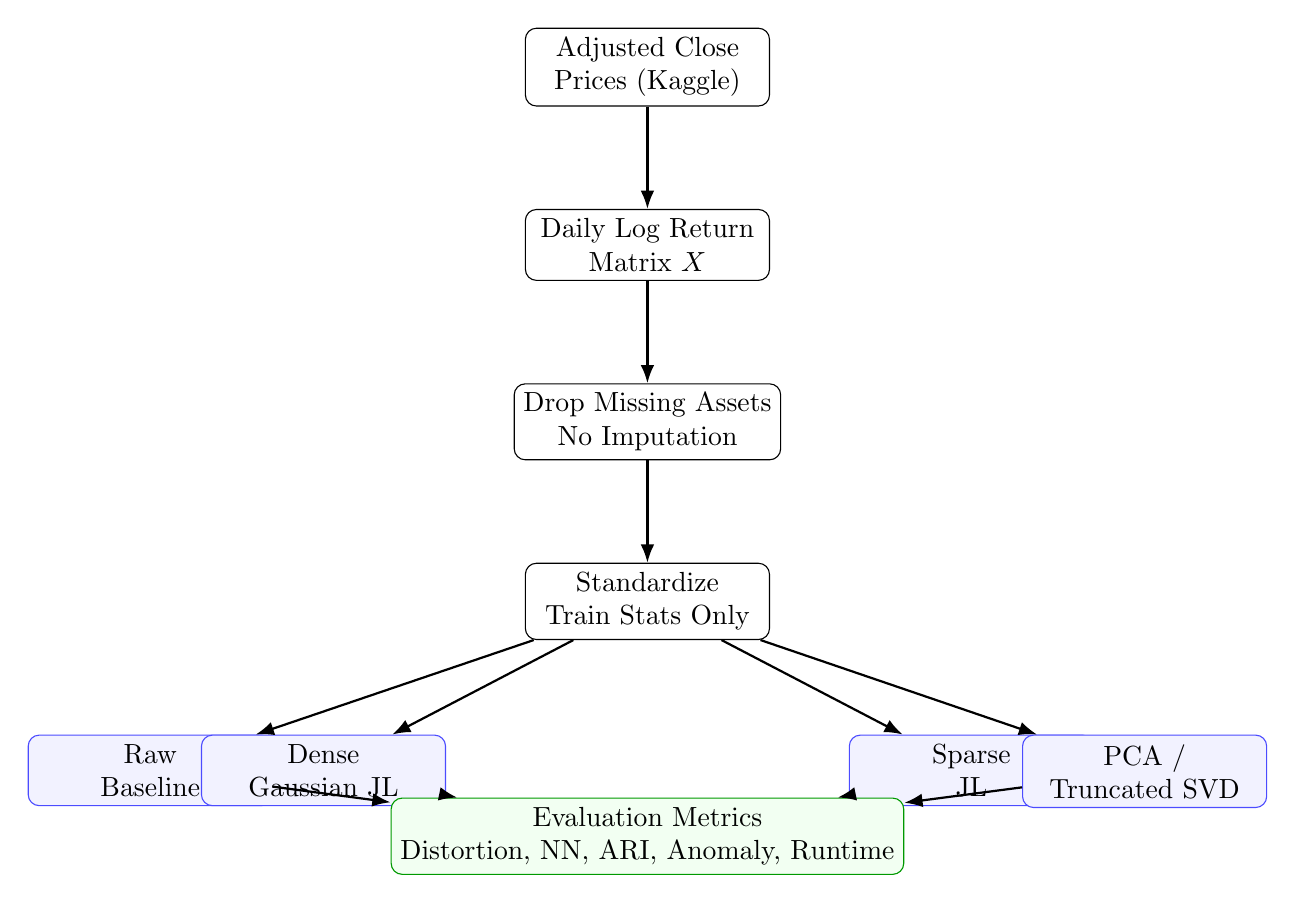
\begin{tikzpicture}[
    node distance=1.3cm,
    box/.style={rectangle, rounded corners, draw=black, align=center, minimum width=3.1cm, minimum height=0.8cm},
    method/.style={rectangle, rounded corners, draw=blue!70, fill=blue!5, align=center, minimum width=3.1cm, minimum height=0.8cm},
    metric/.style={rectangle, rounded corners, draw=green!60!black, fill=green!5, align=center, minimum width=3.1cm, minimum height=0.8cm},
    arrow/.style={-{Latex}, thick}
]

\node[box] (prices) {Adjusted Close\\Prices (Kaggle)};
\node[box, below=of prices] (returns) {Daily Log Return\\Matrix $X$};
\node[box, below=of returns] (clean) {Drop Missing Assets\\No Imputation};
\node[box, below=of clean] (std) {Standardize\\Train Stats Only};

\node[method, below left=1.2cm and 3.2cm of std] (raw) {Raw\\Baseline};
\node[method, below left=1.2cm and 1.0cm of std] (dense) {Dense\\Gaussian JL};
\node[method, below right=1.2cm and 1.0cm of std] (sparse) {Sparse\\JL};
\node[method, below right=1.2cm and 3.2cm of std] (pca) {PCA /\\Truncated SVD};

\node[metric, below=2.0cm of std] (eval) {Evaluation Metrics\\Distortion, NN, ARI, Anomaly, Runtime};

\draw[arrow] (prices) -- (returns);
\draw[arrow] (returns) -- (clean);
\draw[arrow] (clean) -- (std);
\draw[arrow] (std) -- (raw);
\draw[arrow] (std) -- (dense);
\draw[arrow] (std) -- (sparse);
\draw[arrow] (std) -- (pca);

\draw[arrow] (raw) -- (eval);
\draw[arrow] (dense) -- (eval);
\draw[arrow] (sparse) -- (eval);
\draw[arrow] (pca) -- (eval);

\end{tikzpicture}
\caption{Real-data experimental pipeline with strict no-imputation cleaning.}
\end{figure}

\subsection{Raw Baseline}

The raw baseline uses the standardized return vectors directly:
\[
Z_{\text{raw}} = \widetilde{X}.
\]

This is not a compressed representation. It serves as the reference geometry against which all compressed methods are evaluated.

\subsection{Dense Gaussian Johnson--Lindenstrauss Projection}

For dense Gaussian JL, generate a projection matrix:
\[
A \in \mathbb{R}^{N \times k},
\]
with entries:
\[
A_{ij} \sim \mathcal{N}\left(0, \frac{1}{k}\right).
\]

The compressed representation is:
\[
Z_{\text{gaussian}} = \widetilde{X} A.
\]

For each target dimension $k$, the method should be run over 10 random seeds. The report should show the mean and standard deviation of each metric across seeds.

\subsection{Sparse Johnson--Lindenstrauss Projection}

For sparse JL, generate a sparse projection matrix:
\[
S \in \mathbb{R}^{N \times k}.
\]

For each input coordinate $j$, choose $s$ output coordinates uniformly at random and assign random signs. The nonzero entries are scaled as:
\[
S_{j,\ell} \in \left\{ -\frac{1}{\sqrt{s}}, +\frac{1}{\sqrt{s}} \right\}.
\]

All other entries are zero.

The compressed representation is:
\[
Z_{\text{sparse}} = \widetilde{X} S.
\]

The core sparse grid is:
\[
s \in \{1, 3, 5\}.
\]

The primary sparse JL setting should be $s=3$.

\subsection{PCA / Truncated SVD}

PCA is the main data-adaptive low-rank baseline. Fit PCA on training data only:
\[
\text{PCA}_k \leftarrow \text{fit}(X_{\text{train}}).
\]

Then transform train and test:
\[
Z_{\text{train,pca}} = X_{\text{train}} V_k,
\]
\[
Z_{\text{test,pca}} = X_{\text{test}} V_k,
\]
where $V_k \in \mathbb{R}^{N \times k}$ contains the top $k$ principal directions.

PCA should be evaluated at the same $k$ values as JL methods.

\subsection{JL Parameter Grid Search}

The JL parameter grid is the cross-product of the core $k$ grid and the core sparsity grid:
\[
k \in \{5, 10, 20, 30, 50, 100\},
\quad
s \in \{1, 3, 5\}.
\]

Only valid sparse JL combinations should be run:
\[
s \leq k.
\]

\subsubsection{Grid Search Outputs}

The JL grid search should produce:

\begin{itemize}
    \item best sparse JL configuration by distance distortion,
    \item best sparse JL configuration by nearest-neighbor overlap,
    \item best sparse JL configuration by anomaly recall,
    \item runtime-memory tradeoff frontier,
    \item comparison against dense Gaussian JL,
    \item comparison against PCA at the same $k$.
\end{itemize}

\subsection{Fairness Rules}

To make the comparison fair:

\begin{enumerate}
    \item All compressed methods must use the same target dimensions.
    \item PCA must be fit on training data only.
    \item Standardization must use training statistics only.
    \item Random projection methods must be averaged across 10 random seeds.
    \item Evaluation should be performed primarily on the test set.
    \item The raw test-set geometry is the reference geometry.
    \item COVID diagnostic experiments must clearly state whether PCA was fit on the primary chronological training set or the pre-COVID training set.
\end{enumerate}

% ============================================================
\section{Evaluation Metrics}

\subsection{Metric 1: Pairwise Distance Distortion}

For sampled pairs of test days $(i,j)$, compute the raw-space distance:
\[
d_{ij} = \|X_i - X_j\|_2.
\]

For a compressed representation $Z$, compute:
\[
\hat{d}_{ij} = \|Z_i - Z_j\|_2.
\]

The multiplicative distortion is:
\[
\rho_{ij} = \frac{\hat{d}_{ij}}{d_{ij}}.
\]

A perfect distance-preserving embedding would have:
\[
\rho_{ij} = 1.
\]

Report the following:

\begin{itemize}
    \item mean absolute distortion:
    \[
    \frac{1}{M}\sum_{(i,j)} |\rho_{ij} - 1|,
    \]
    \item median distortion,
    \item 95th percentile absolute distortion,
    \item distribution plots of $\rho_{ij}$,
    \item COVID vs. non-COVID distortion comparison.
\end{itemize}

This is the most direct metric connected to the Johnson--Lindenstrauss perspective.

\subsection{Metric 2: Nearest-Neighbor Preservation}

For each test day $i$, compute its $m$ nearest neighbors in raw space:
\[
\mathcal{N}^{\text{raw}}_m(i).
\]

Then compute its $m$ nearest neighbors in compressed space:
\[
\mathcal{N}^{\text{comp}}_m(i).
\]

The neighbor overlap is:
\[
\text{NNOverlap}_m(i)
=
\frac{
\left|
\mathcal{N}^{\text{raw}}_m(i)
\cap
\mathcal{N}^{\text{comp}}_m(i)
\right|
}{m}.
\]

Use:
\[
m \in \{5, 10\}.
\]

Report average top-5 and top-10 nearest-neighbor overlap across all test days and across COVID-specific slices.

\subsection{Metric 3: Clustering Stability}

The goal is to test whether compressed representations preserve market-state clusters.

Procedure:

\begin{enumerate}
    \item Run KMeans clustering on raw test data.
    \item Run KMeans clustering on compressed test data.
    \item Compare cluster labels using Adjusted Rand Index.
\end{enumerate}

Use cluster counts:
\[
C \in \{3, 5, 8\}.
\]

The main clustering metric is Adjusted Rand Index:
\[
\text{ARI} \in [-1, 1],
\]
where larger values indicate stronger agreement between clusterings.

Report:

\begin{itemize}
    \item ARI by method and $k$,
    \item average ARI across cluster counts,
    \item sensitivity to cluster count,
    \item COVID vs. non-COVID ARI.
\end{itemize}

\subsection{Metric 4: Unusual Market Day Preservation}

Define an anomaly score in raw space:
\[
a_i = \|X_i\|_2.
\]

A test day is considered unusual if its raw anomaly score lies in the top 5\%:
\[
i \in \mathcal{A}_{\text{raw}}.
\]

For compressed representation $Z$, compute:
\[
\hat{a}_i = \|Z_i\|_2.
\]

Let $\mathcal{A}_{\text{comp}}$ be the top 5\% of days according to compressed anomaly scores.

Report:

\[
\text{Recall@5\%}
=
\frac{
|\mathcal{A}_{\text{raw}} \cap \mathcal{A}_{\text{comp}}|
}{
|\mathcal{A}_{\text{raw}}|
}.
\]

Also report:

\begin{itemize}
    \item precision@5\%,
    \item anomaly-score correlation,
    \item top-10 unusual day overlap,
    \item COVID-only anomaly preservation.
\end{itemize}

\subsection{Metric 5: Runtime and Sparsity}

Since sparse JL is motivated by efficiency, the implementation should also record:

\begin{itemize}
    \item projection matrix construction time,
    \item transform runtime,
    \item metric computation runtime,
    \item number of nonzero entries in the projection matrix,
    \item memory footprint of the projection matrix,
    \item total end-to-end experiment time.
\end{itemize}

This allows the final report to discuss whether sparse JL is practically attractive even if PCA performs better on some accuracy metrics.

% ============================================================
\section{Synthetic Factor-Model Experiment}

\subsection{Purpose}

The synthetic experiment is essential for the low-rank factor structure question. Real financial data may be noisy and difficult to interpret. Synthetic factor data allows us to control:

\begin{itemize}
    \item true factor rank,
    \item noise level,
    \item factor strength,
    \item dimensionality.
\end{itemize}

This gives a clean way to answer:

\begin{quote}
When data is strongly low-rank, does PCA clearly dominate sparse JL? As noise increases or the factor structure weakens, does sparse JL become more competitive?
\end{quote}

\subsection{Synthetic Data Model}

Generate:
\[
X = F B^\top + E,
\]
where:

\begin{itemize}
    \item $X \in \mathbb{R}^{T \times N}$ is the synthetic return matrix,
    \item $F \in \mathbb{R}^{T \times r}$ contains latent factor returns,
    \item $B \in \mathbb{R}^{N \times r}$ contains asset factor loadings,
    \item $E \in \mathbb{R}^{T \times N}$ is idiosyncratic noise,
    \item $r$ is the true latent factor rank.
\end{itemize}

A simple implementation is:
\[
F_{t,j} \sim \mathcal{N}(0,1),
\]
\[
B_{i,j} \sim \mathcal{N}(0,1),
\]
\[
E_{t,i} \sim \mathcal{N}(0,\sigma^2).
\]

Then:
\[
X = F B^\top + E.
\]

\subsection{Synthetic Experimental Grid}

Use:

\[
r \in \{3, 5, 10, 20\},
\]
\[
\sigma \in \{0.1, 0.5, 1.0\}.
\]

For each $(r,\sigma)$ pair, evaluate all methods at:
\[
k \in \{5, 10, 20, 30, 50, 100\}.
\]

The expected behavior is:

\begin{itemize}
    \item When $r$ is small and $\sigma$ is low, PCA should perform extremely well.
    \item When $\sigma$ increases, the advantage of PCA may shrink.
    \item When $k$ is much larger than $r$, random projections may become more competitive.
    \item Sparse JL may provide a useful efficiency tradeoff if its metrics are close to dense JL or PCA.
\end{itemize}

\subsection{Synthetic Experiment Diagram}

\begin{figure}[H]
\centering
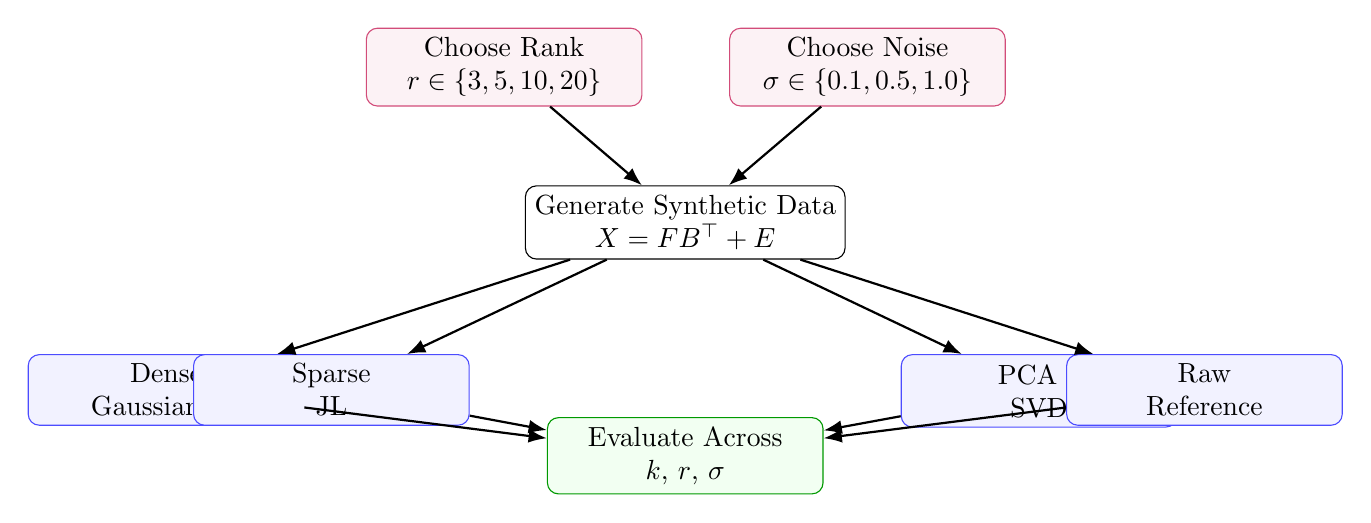
\begin{tikzpicture}[
    node distance=1.1cm,
    box/.style={rectangle, rounded corners, draw=black, align=center, minimum width=3.5cm, minimum height=0.8cm},
    param/.style={rectangle, rounded corners, draw=purple!70, fill=purple!5, align=center, minimum width=3.5cm, minimum height=0.8cm},
    method/.style={rectangle, rounded corners, draw=blue!70, fill=blue!5, align=center, minimum width=3.5cm, minimum height=0.8cm},
    metric/.style={rectangle, rounded corners, draw=green!60!black, fill=green!5, align=center, minimum width=3.5cm, minimum height=0.8cm},
    arrow/.style={-{Latex}, thick}
]

\node[param] (rank) {Choose Rank\\$r \in \{3,5,10,20\}$};
\node[param, right=of rank] (noise) {Choose Noise\\$\sigma \in \{0.1,0.5,1.0\}$};

\node[box, below=1.0cm of rank, xshift=2.3cm] (gen) {Generate Synthetic Data\\$X = F B^\top + E$};

\node[method, below left=1.2cm and 2.8cm of gen] (dense) {Dense\\Gaussian JL};
\node[method, below left=1.2cm and 0.7cm of gen] (sparse) {Sparse\\JL};
\node[method, below right=1.2cm and 0.7cm of gen] (pca) {PCA /\\SVD};
\node[method, below right=1.2cm and 2.8cm of gen] (raw) {Raw\\Reference};

\node[metric, below=2.0cm of gen] (eval) {Evaluate Across\\$k$, $r$, $\sigma$};

\draw[arrow] (rank) -- (gen);
\draw[arrow] (noise) -- (gen);

\draw[arrow] (gen) -- (dense);
\draw[arrow] (gen) -- (sparse);
\draw[arrow] (gen) -- (pca);
\draw[arrow] (gen) -- (raw);

\draw[arrow] (dense) -- (eval);
\draw[arrow] (sparse) -- (eval);
\draw[arrow] (pca) -- (eval);
\draw[arrow] (raw) -- (eval);

\end{tikzpicture}
\caption{Synthetic factor-model experiment.}
\end{figure}

% ============================================================
\section{Parallel Execution Plan}

\subsection{Why Parallelization Is Needed}

The experiment grid is large. A naive linear implementation would run:

\begin{itemize}
    \item multiple methods,
    \item multiple target dimensions,
    \item multiple sparse JL sparsity values,
    \item multiple random seeds,
    \item multiple evaluation slices,
    \item multiple synthetic ranks,
    \item multiple synthetic noise levels,
    \item multiple metrics.
\end{itemize}

Most experiment configurations are embarrassingly parallel. For example, sparse JL with $(k=20, s=3, seed=4)$ can be evaluated independently from sparse JL with $(k=50, s=5, seed=7)$. Synthetic experiments are also independent across $(r,\sigma,k,s,seed)$.

Therefore, the implementation should be designed with a parallel execution backend.

\subsection{Recommended Backend Strategy}

The implementation should support two execution backends:

\begin{enumerate}
    \item \textbf{Local backend:} runs experiments sequentially or with standard multiprocessing. This is required for debugging and reproducibility.

    \item \textbf{Ray backend:} runs independent experiment configurations in parallel. This is preferred for the full grid search and synthetic experiments.
\end{enumerate}

Ray is useful if:

\begin{itemize}
    \item synthetic rank/noise experiments are included,
    \item COVID-specific slices are evaluated separately,
    \item repeated random seeds are used,
    \item figure generation is separated from metric computation.
\end{itemize}

Ray is not strictly necessary for a minimal version, but the code should be designed so that Ray can be enabled without rewriting the experiment logic.

\subsection{Parallelization Unit}

The atomic unit of parallel work should be an experiment configuration:

\begin{verbatim}
ExperimentConfig(
    dataset_type,
    evaluation_slice,
    method,
    k,
    sparse_s,
    seed,
    synthetic_rank,
    synthetic_noise,
    metric_bundle
)
\end{verbatim}

Each worker should:

\begin{enumerate}
    \item load or receive the prepared dataset,
    \item construct the projection or fit PCA if needed,
    \item transform the selected evaluation data,
    \item compute the requested metrics,
    \item return a structured result dictionary,
    \item save intermediate outputs only if requested.
\end{enumerate}

\subsection{Parallel Execution Diagram}

\begin{figure}[H]
\centering
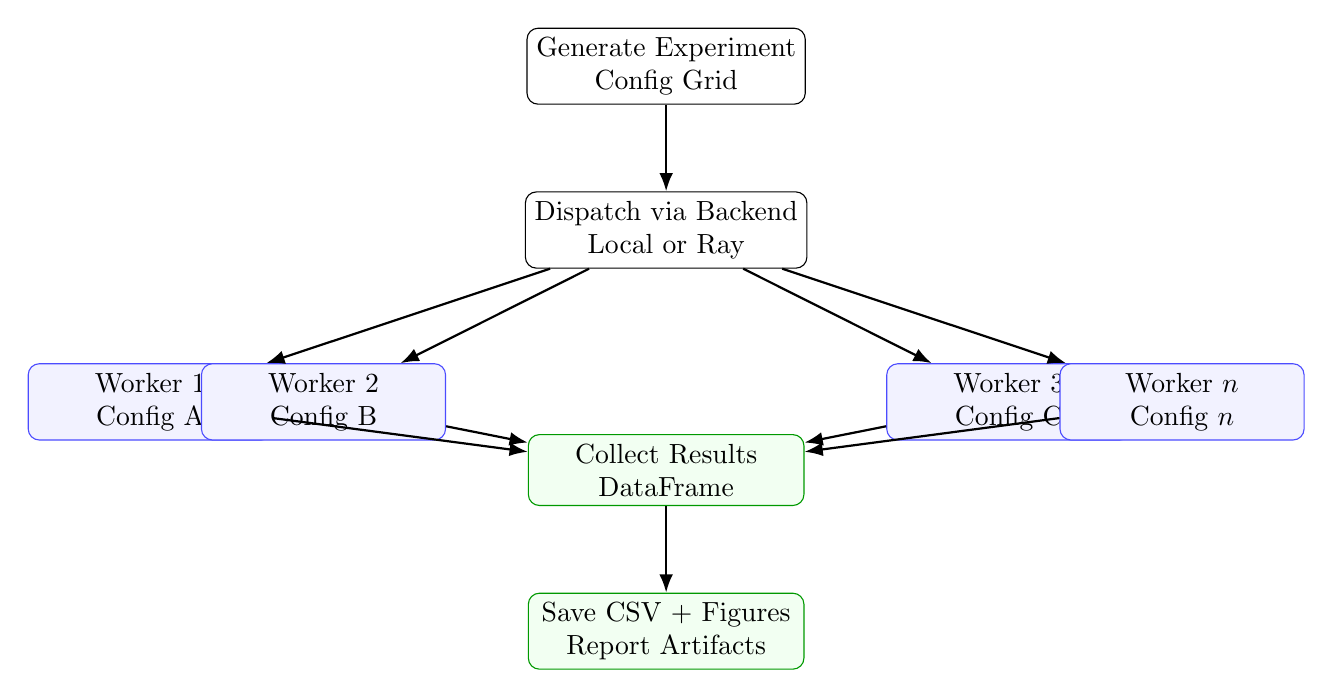
\begin{tikzpicture}[
    node distance=1.1cm,
    box/.style={rectangle, rounded corners, draw=black, align=center, minimum width=3.4cm, minimum height=0.75cm},
    worker/.style={rectangle, rounded corners, draw=blue!70, fill=blue!5, align=center, minimum width=3.1cm, minimum height=0.75cm},
    output/.style={rectangle, rounded corners, draw=green!60!black, fill=green!5, align=center, minimum width=3.5cm, minimum height=0.75cm},
    arrow/.style={-{Latex}, thick}
]

\node[box] (config) {Generate Experiment\\Config Grid};
\node[box, below=of config] (dispatch) {Dispatch via Backend\\Local or Ray};

\node[worker, below left=1.2cm and 3.2cm of dispatch] (w1) {Worker 1\\Config A};
\node[worker, below left=1.2cm and 1.0cm of dispatch] (w2) {Worker 2\\Config B};
\node[worker, below right=1.2cm and 1.0cm of dispatch] (w3) {Worker 3\\Config C};
\node[worker, below right=1.2cm and 3.2cm of dispatch] (w4) {Worker $n$\\Config $n$};

\node[output, below=2.1cm of dispatch] (collect) {Collect Results\\DataFrame};
\node[output, below=of collect] (save) {Save CSV + Figures\\Report Artifacts};

\draw[arrow] (config) -- (dispatch);
\draw[arrow] (dispatch) -- (w1);
\draw[arrow] (dispatch) -- (w2);
\draw[arrow] (dispatch) -- (w3);
\draw[arrow] (dispatch) -- (w4);

\draw[arrow] (w1) -- (collect);
\draw[arrow] (w2) -- (collect);
\draw[arrow] (w3) -- (collect);
\draw[arrow] (w4) -- (collect);

\draw[arrow] (collect) -- (save);

\end{tikzpicture}
\caption{Parallel experiment execution design.}
\end{figure}

\subsection{Required Backend Interface}

The implementation should expose a backend-agnostic runner:

\begin{lstlisting}[language=Python]
def run_experiment_grid(configs, backend="local", num_cpus=None):
    """
    Runs a list of ExperimentConfig objects.

    backend:
        "local" -> sequential or multiprocessing fallback
        "ray"   -> Ray-based parallel execution

    Returns:
        pandas.DataFrame with one row per experiment result.
    """
\end{lstlisting}

The local and Ray backends should produce identical result schemas.

\subsection{Ray-Style Pseudocode}

\begin{lstlisting}[language=Python]
@ray.remote
def run_single_config_remote(config, shared_data_ref):
    data = ray.get(shared_data_ref)
    return run_single_config(config, data)

def run_with_ray(configs, prepared_data, num_cpus=None):
    ray.init(num_cpus=num_cpus, ignore_reinit_error=True)
    shared_data_ref = ray.put(prepared_data)

    futures = [
        run_single_config_remote.remote(config, shared_data_ref)
        for config in configs
    ]

    results = ray.get(futures)
    return pd.DataFrame(results)
\end{lstlisting}

\subsection{Parallelization Risks}

\begin{longtable}{p{0.25\linewidth} p{0.35\linewidth} p{0.30\linewidth}}
\caption{Parallelization Risks and Mitigations} \\
\toprule
\textbf{Risk} & \textbf{Why It Matters} & \textbf{Mitigation} \\
\midrule
\endfirsthead

\toprule
\textbf{Risk} & \textbf{Why It Matters} & \textbf{Mitigation} \\
\midrule
\endhead

Ray overhead exceeds benefit & Small datasets may not need distributed execution & Keep local backend; use Ray only when grid is large \\

Random seeds inconsistent & Parallel execution can make randomness harder to reproduce & Store seed in every config and result row \\

Large data copied to workers & Memory overhead can increase & Use shared object store via \texttt{ray.put}; avoid repeated copies \\

Race conditions in output files & Multiple workers may write to same path & Workers return results; central process writes outputs \\

Difficult debugging & Parallel traces are harder to inspect & Debug first using local backend on small grid \\

Environment mismatch & Ray may not be installed on all machines & Make Ray optional dependency; local backend required \\

\bottomrule
\end{longtable}

% ============================================================
\section{Market Regime Analysis}

\subsection{Purpose}

Financial data changes across regimes. A method that works well in calm periods may fail during high-volatility periods. To address this, the real-data test set should be divided into volatility regimes.

\subsection{Market Return and Rolling Volatility}

Define the equal-weighted market return:
\[
m_t = \frac{1}{N} \sum_{i=1}^{N} X_{t,i}.
\]

Compute 20-day rolling volatility:
\[
v_t = \operatorname{std}(m_{t-19}, \ldots, m_t).
\]

Divide test days into three groups:

\begin{itemize}
    \item low-volatility regime,
    \item medium-volatility regime,
    \item high-volatility regime.
\end{itemize}

The split can be based on volatility tertiles.

\subsection{Regime-Specific Evaluation}

For each volatility regime, recompute:

\begin{itemize}
    \item pairwise distance distortion,
    \item nearest-neighbor preservation,
    \item anomaly recall,
    \item anomaly-score correlation.
\end{itemize}

This directly supports the third research question: whether volatility regimes affect the success or failure of sparse JL.

% ============================================================
\section{Required Figure Plan}

\subsection{Purpose of the Expanded Figure Set}

The final report should include enough figures to make the data behavior and method comparisons interpretable. The goal is not to add plots for volume. The goal is to make every major conclusion visually defensible.

The implementation must generate at least 40 figures. The final written report can include the most important figures in the main body and move the rest to an appendix.

\subsection{Figure Generation Principles}

Every figure should satisfy the following rules:

\begin{enumerate}
    \item The filename must be deterministic.
    \item The plot title must identify the dataset slice, method family, and metric.
    \item Axes must be labeled clearly.
    \item If random seeds are involved, plot mean with variability bands or error bars.
    \item The underlying CSV used for each figure must be saved.
    \item Figures should be generated from saved result files, not directly from transient in-memory experiment state.
\end{enumerate}

\subsection{Minimum Figure Catalogue}

\begin{longtable}{p{0.05\linewidth} p{0.27\linewidth} p{0.22\linewidth} p{0.36\linewidth}}
\caption{Required Figure Catalogue: At Least 40 Figures} \\
\toprule
\textbf{\#} & \textbf{Filename} & \textbf{Category} & \textbf{Purpose} \\
\midrule
\endfirsthead

\toprule
\textbf{\#} & \textbf{Filename} & \textbf{Category} & \textbf{Purpose} \\
\midrule
\endhead

1 & fig\_price\_coverage.png & Data diagnostic & Shows final asset coverage after missing-data filtering \\
2 & fig\_missing\_asset\_drop\_summary.png & Data diagnostic & Shows which assets were dropped and replaced \\
3 & fig\_return\_distribution\_all.png & Data diagnostic & Distribution of daily log returns across all assets \\
4 & fig\_asset\_volatility\_distribution.png & Data diagnostic & Shows cross-sectional variation in asset volatility \\
5 & fig\_correlation\_heatmap.png & Data diagnostic & Visualizes cross-sectional correlation structure \\
6 & fig\_average\_correlation\_over\_time.png & Data diagnostic & Tracks market-wide correlation through time \\
7 & fig\_market\_return\_timeline.png & Data diagnostic & Shows equal-weighted market return over time \\
8 & fig\_rolling\_volatility\_timeline.png & Regime diagnostic & Shows 20-day rolling market volatility \\
9 & fig\_regime\_labels\_timeline.png & Regime diagnostic & Marks low, medium, high volatility regimes \\
10 & fig\_covid\_stress\_window\_timeline.png & COVID diagnostic & Highlights COVID-stress window on return timeline \\
11 & fig\_pca\_explained\_variance.png & PCA diagnostic & Cumulative explained variance vs number of components \\
12 & fig\_pca\_scree\_plot.png & PCA diagnostic & Individual explained variance by component \\
13 & fig\_pca\_top\_component\_loadings.png & PCA diagnostic & Interprets first principal component exposure \\
14 & fig\_pca\_2d\_projection.png & PCA diagnostic & Two-dimensional visualization of market states \\
15 & fig\_raw\_distance\_distribution.png & Raw geometry & Distribution of pairwise distances in raw space \\
16 & fig\_distortion\_vs\_k\_main.png & Main metric & Distance distortion vs $k$ for core methods \\
17 & fig\_distortion\_boxplot\_by\_method.png & Main metric & Distribution of distance distortion by method \\
18 & fig\_distortion\_dense\_vs\_sparse.png & JL comparison & Compares dense Gaussian JL against sparse JL \\
19 & fig\_distortion\_sparse\_sweep.png & JL grid & Shows sparse JL distortion across $k$ and $s$ \\
20 & fig\_nn5\_overlap\_vs\_k.png & Main metric & Top-5 nearest-neighbor preservation vs $k$ \\
21 & fig\_nn10\_overlap\_vs\_k.png & Main metric & Top-10 nearest-neighbor preservation vs $k$ \\
22 & fig\_nn\_heatmap\_method\_k.png & Main metric & Heatmap of nearest-neighbor overlap by method and $k$ \\
23 & fig\_clustering\_ari\_vs\_k.png & Main metric & Clustering ARI vs $k$ \\
24 & fig\_clustering\_ari\_by\_clusters.png & Main metric & ARI sensitivity to cluster count \\
25 & fig\_cluster\_embedding\_comparison.png & Clustering diagnostic & Visual comparison of raw/PCA/JL clusters \\
26 & fig\_anomaly\_recall\_vs\_k.png & Main metric & Top-5\% anomaly recall vs $k$ \\
27 & fig\_anomaly\_score\_correlation.png & Main metric & Correlation between raw and compressed anomaly scores \\
28 & fig\_top10\_anomaly\_rank\_comparison.png & Main metric & Rank preservation of top-10 unusual days \\
29 & fig\_runtime\_transform\_vs\_k.png & Runtime & Transform runtime vs $k$ \\
30 & fig\_projection\_memory\_vs\_k.png & Runtime & Projection matrix memory footprint vs $k$ \\
31 & fig\_sparse\_nnz\_vs\_dense\_nnz.png & Runtime & Nonzero count comparison for dense vs sparse JL \\
32 & fig\_runtime\_accuracy\_frontier.png & Runtime & Accuracy-runtime tradeoff frontier \\
33 & fig\_full\_including\_covid\_distortion.png & COVID & Distance distortion including COVID \\
34 & fig\_excluding\_covid\_distortion.png & COVID & Distance distortion excluding COVID \\
35 & fig\_covid\_only\_distortion.png & COVID & Distance distortion only during COVID-stress window \\
36 & fig\_covid\_nn\_overlap.png & COVID & Nearest-neighbor preservation during COVID-stress window \\
37 & fig\_covid\_anomaly\_recall.png & COVID & Anomaly recall during COVID-stress window \\
38 & fig\_covid\_top10\_unusual\_days.png & COVID & Top-10 unusual COVID days under raw and compressed spaces \\
39 & fig\_covid\_vs\_noncovid\_metric\_delta.png & COVID & Difference between COVID and non-COVID performance \\
40 & fig\_regime\_distortion\_comparison.png & Regime & Distortion across low/medium/high volatility regimes \\
41 & fig\_regime\_nn\_comparison.png & Regime & Nearest-neighbor overlap by volatility regime \\
42 & fig\_regime\_anomaly\_comparison.png & Regime & Anomaly recall by volatility regime \\
43 & fig\_synthetic\_distortion\_rank\_noise\_heatmap.png & Synthetic & Distance distortion by true rank and noise \\
44 & fig\_synthetic\_nn\_rank\_noise\_heatmap.png & Synthetic & NN overlap by true rank and noise \\
45 & fig\_synthetic\_pca\_advantage\_heatmap.png & Synthetic & Where PCA beats sparse JL most clearly \\
46 & fig\_synthetic\_sparsejl\_competitive\_region.png & Synthetic & Regions where sparse JL approaches PCA \\
47 & fig\_synthetic\_noise\_sensitivity.png & Synthetic & Performance degradation as noise increases \\
48 & fig\_synthetic\_rank\_sensitivity.png & Synthetic & Performance degradation as true rank increases \\
49 & fig\_jl\_seed\_variance.png & Robustness & Variance of JL metrics across random seeds \\
50 & fig\_best\_method\_by\_metric.png & Summary & Best method for each metric and $k$ \\
\bottomrule
\end{longtable}

\subsection{Main-Report vs. Appendix Figures}

The final written report should not place all 50 figures in the main body. The recommended split is:

\begin{itemize}
    \item \textbf{Main report:} 10--15 most important figures.
    \item \textbf{Appendix:} remaining diagnostic and sensitivity figures.
\end{itemize}

The main report should prioritize:

\begin{enumerate}
    \item PCA explained variance.
    \item Main distortion vs $k$.
    \item NN overlap vs $k$.
    \item Anomaly recall vs $k$.
    \item Runtime-accuracy frontier.
    \item COVID-only distortion.
    \item COVID-only anomaly recall.
    \item Synthetic PCA advantage heatmap.
    \item Synthetic sparse JL competitive region.
    \item Regime-specific comparison.
\end{enumerate}

% ============================================================
\section{Expected Results and Interpretation}

\subsection{Expected Result 1: PCA Dominates Under Strong Low-Rank Structure}

If financial returns have strong low-rank factor structure, PCA should perform well at small $k$. This would likely appear as:

\begin{itemize}
    \item high explained variance at low $k$,
    \item strong nearest-neighbor preservation,
    \item high clustering stability,
    \item good anomaly preservation.
\end{itemize}

This would support the view that data-adaptive compression is superior when the structure is strongly low-rank.

\subsection{Expected Result 2: Sparse JL Becomes Competitive as $k$ Increases}

Sparse JL may perform poorly at very small $k$ but improve as $k$ increases. If sparse JL approaches dense Gaussian JL or PCA at moderate dimensions, then it may be attractive because of its computational efficiency.

This would support the claim that sparse JL can be a practical compression tool even when it is not the best purely statistical method.

\subsection{Expected Result 3: Noise Weakens PCA's Advantage}

In synthetic data, when noise level $\sigma$ increases, the benefit of PCA may decrease. PCA is optimal for capturing variance, but if much of the variance is noise, its advantage may become less meaningful for preserving neighborhoods or anomaly structure.

\subsection{Expected Result 4: COVID and High-Volatility Regimes May Be Harder to Preserve}

During high-volatility periods, market structure may change quickly. Compression methods may struggle more in these regimes. The report should examine whether:

\begin{itemize}
    \item PCA remains robust,
    \item sparse JL degrades sharply,
    \item anomaly recall differs across COVID and non-COVID periods,
    \item nearest-neighbor structure is less stable during the COVID-stress window.
\end{itemize}

% ============================================================
\section{Implementation Output Contract}

The final agent implementation should produce a reproducible project with the following structure.

\begin{verbatim}
project_root/
    README.md
    requirements.txt
    pyproject.toml                    # optional but preferred

    configs/
        experiment_config.yaml        # records pinned Kaggle version
        figure_catalog.yaml

    data/
        raw/
            sp500_prices.csv          # pinned Kaggle dump
        processed/
            returns_matrix.csv
            standardized_returns_train.csv
            standardized_returns_test.csv
            asset_list.csv
            date_index.csv
            preprocessing_report.json

    src/
        data_loader.py                # loads Kaggle CSV, yfinance fallback
        preprocessing.py
        projections.py
        pca_baseline.py
        metrics.py
        synthetic_data.py
        experiment_config.py
        experiment_runner.py
        parallel_backend.py
        experiments_real.py
        experiments_synthetic.py
        experiments_covid.py
        experiments_regime.py
        plotting.py
        utils.py

    scripts/
        run_data_pipeline.py
        run_real_experiments.py
        run_synthetic_experiments.py
        run_covid_experiments.py
        run_regime_experiments.py
        generate_figures.py
        run_all.py

    notebooks/
        exploratory_analysis.ipynb
        final_results.ipynb

    results/
        real_distance_distortion.csv
        real_nearest_neighbor_overlap.csv
        real_clustering_stability.csv
        real_anomaly_preservation.csv
        real_runtime_memory.csv
        jl_grid_search_results.csv
        synthetic_results.csv
        covid_results.csv
        regime_results.csv

    figures/
        fig_*.png

    report/
        final_report.tex
        references.bib
\end{verbatim}

\subsection{Minimum Required Tables}

The final report should include the following tables:

\begin{enumerate}
    \item Dataset summary table (including pinned Kaggle version).
    \item Missing-data drop-and-replacement table.
    \item Preprocessing summary table.
    \item Method comparison table.
    \item Main real-data metric table.
    \item JL grid-search summary table.
    \item COVID vs. non-COVID metric table.
    \item Synthetic factor-model result table.
    \item Runtime and memory comparison table.
    \item Final recommendation table.
\end{enumerate}

\subsection{Minimum Required Figures}

The implementation must generate at least 40 figures, following the figure catalogue in Section 11. The report should include the strongest figures in the main body and place the remaining figures in the appendix.

% ============================================================
\section{Implementation Phases}

\subsection{Phase 1: Finalize Design}

Before coding begins, the team must finalize:

\begin{itemize}
    \item asset universe (S\&P 500 today's constituents),
    \item reserve universe for replacement assets,
    \item data source (Kaggle dataset name and version pin),
    \item date range,
    \item strict no-imputation missing-data policy,
    \item core target-dimension grid,
    \item sparse JL sparsity grid,
    \item random seed count,
    \item COVID stress window,
    \item anomaly definition,
    \item Ray usage policy,
    \item exact deliverables.
\end{itemize}

\subsection{Phase 2: Data Pipeline}

Tasks:

\begin{enumerate}
    \item Download adjusted close prices from the pinned Kaggle dataset (yfinance fallback if unavailable).
    \item Record the Kaggle dataset version and download date in \texttt{configs/experiment\_config.yaml}.
    \item Build a clean price matrix.
    \item Drop assets with missing values.
    \item Replace dropped assets from reserve universe if needed.
    \item Confirm that final price matrix has no missing values.
    \item Run validation cross-check on a sample of tickers against a second source.
    \item Compute daily log returns.
    \item Split chronologically into train and test.
    \item Fit standardization parameters on train.
    \item Transform train and test.
    \item Save all processed artifacts.
\end{enumerate}

\subsection{Phase 3: Compression Methods}

Tasks:

\begin{enumerate}
    \item Implement raw baseline.
    \item Implement dense Gaussian JL.
    \item Implement sparse JL with core sparsity grid.
    \item Implement PCA / truncated SVD.
    \item Ensure all methods expose a common interface.
\end{enumerate}

The common interface should behave conceptually as:

\begin{verbatim}
fit(X_train)
transform(X)
fit_transform(X_train)
\end{verbatim}

For random projection methods, \texttt{fit} generates and stores the projection matrix.

\subsection{Phase 4: Metrics}

Tasks:

\begin{enumerate}
    \item Implement pairwise distance distortion.
    \item Implement nearest-neighbor overlap.
    \item Implement clustering ARI.
    \item Implement anomaly recall.
    \item Implement anomaly-score correlation.
    \item Implement top-10 unusual day rank preservation.
    \item Implement runtime and memory logging.
\end{enumerate}

\subsection{Phase 5: Parallel Experiment Runner}

Tasks:

\begin{enumerate}
    \item Define \texttt{ExperimentConfig}.
    \item Generate experiment grid.
    \item Implement local backend.
    \item Implement Ray backend.
    \item Ensure both backends return identical result schemas.
    \item Add deterministic random seed handling.
    \item Save all results centrally after worker completion.
\end{enumerate}

\subsection{Phase 6: Real-Data Experiments}

For each method and each target dimension $k$:

\begin{enumerate}
    \item Fit method on train if needed.
    \item Transform test data.
    \item Compute all metrics.
    \item Save results.
\end{enumerate}

For JL methods, repeat across 10 random seeds and aggregate mean and standard deviation.

\subsection{Phase 7: COVID Experiments}

Run the same metric suite for:

\begin{enumerate}
    \item full sample including COVID,
    \item full sample excluding COVID,
    \item COVID-stress-only window,
    \item optional COVID-year diagnostic window.
\end{enumerate}

The COVID diagnostic protocol should also fit PCA and standardization using pre-COVID data only when performing the out-of-sample COVID stress analysis.

\subsection{Phase 8: Synthetic Experiments}

For each synthetic rank $r$, noise level $\sigma$, method, and dimension $k$:

\begin{enumerate}
    \item Generate synthetic data.
    \item Split into train and test.
    \item Standardize using train statistics.
    \item Apply compression methods.
    \item Compute metrics.
    \item Save results.
\end{enumerate}

\subsection{Phase 9: Figure Generation}

Tasks:

\begin{enumerate}
    \item Read saved result CSV files.
    \item Generate all required figures in the figure catalogue.
    \item Save figures to \texttt{figures/}.
    \item Save any figure-specific source data if needed.
    \item Produce a figure manifest file.
\end{enumerate}

\subsection{Phase 10: Analysis and Report}

Tasks:

\begin{enumerate}
    \item Generate all required tables.
    \item Interpret results around the low-rank factor structure question.
    \item Discuss whether sparse JL is competitive with PCA.
    \item Discuss computational tradeoffs.
    \item Discuss COVID-specific findings.
    \item Discuss synthetic factor-model findings.
    \item Write limitations (including survivorship bias from today's S\&P 500 backfill).
    \item Prepare final report.
\end{enumerate}

% ============================================================
\section{Risks and Mitigations}\label{sec:risks}

\begin{longtable}{p{0.25\linewidth} p{0.35\linewidth} p{0.30\linewidth}}
\caption{Risks and Mitigation Strategies} \\
\toprule
\textbf{Risk} & \textbf{Why It Matters} & \textbf{Mitigation} \\
\midrule
\endfirsthead

\toprule
\textbf{Risk} & \textbf{Why It Matters} & \textbf{Mitigation} \\
\midrule
\endhead

Missing data across assets & Kaggle CSV may have gaps for tickers added or removed mid-period & Drop those tickers and replace from a reserve list of next-ranked S\&P 500 names; document drops in \texttt{preprocessing\_report.json} \\

Survivorship bias (today's S\&P 500 backfilled) & Companies in the 2014 S\&P 500 that were later acquired, bankrupt, or demoted (e.g.\ Time Warner, Sprint, Allergan) are excluded; results may be biased toward calm-regime survivors & State explicitly in Section~14 (Limitations) and final report; project is about compression geometry, not trading P\&L; trade-off accepted in lieu of paid CRSP/WRDS access \\

Kaggle dataset quality & Community-maintained data may have silent adjustment errors or stale rows & Pin a specific dataset version; cross-check a random sample of tickers against yfinance or Stooq; document discrepancies \\

Kaggle dataset unavailable at run time & Dataset can be removed or renamed by the maintainer & Implement yfinance fallback that loads the same fixed ticker list and produces an identical schema \\

No-imputation policy reduces universe size & Strict filtering may remove many assets & Use reserve list and target a realistic final $N$; report final $N$ alongside drop count \\

PCA data leakage & Fitting PCA on all data would inflate test performance & Fit PCA only on training data \\

Standardization leakage & Using full-sample mean/std leaks test information & Compute standardization parameters on train only \\

COVID leakage & COVID may fall inside training period under 70/30 split & Add pre-COVID diagnostic protocol \\

Randomness in JL & Single-seed results may be unstable & Use 10 seeds and report mean/std \\

Too many experimental branches & Project may become too broad & Restrict to core grid only; extras go to optional appendix \\

Weak real-data conclusions & Real data may be noisy or ambiguous & Use synthetic factor-model experiment to isolate low-rank effects \\

Anomaly definition too vague & Results may be hard to defend & Define unusual days as top 5\% by raw market-state norm \\

Runtime results inconsistent & Machine-dependent measurements can vary & Use relative comparisons and average repeated runs \\

Ray overhead & Parallelization may not help small grids & Keep local backend; use Ray when grid is large \\

Too many figures & Report may become cluttered & Put only strongest figures in main report; move rest to appendix \\

\bottomrule
\end{longtable}

% ============================================================
\section{Team Decisions Required Before Implementation}

The team should approve or modify the following items before the plan is converted into an execution prompt.

\begin{table}[H]
\centering
\caption{Pre-Implementation Decision Checklist}
\begin{tabular}{p{0.45\linewidth} p{0.40\linewidth}}
\toprule
\textbf{Decision} & \textbf{Recommended Choice} \\
\midrule
Asset universe & S\&P 500 today's constituents ($\sim$500 names); survivorship-biased \\
Data source & Kaggle: \texttt{andrewmvd/sp-500-stocks} (Larxel), pinned dataset version; yfinance fallback \\
Validation cross-check & Compare 5--10 random tickers against yfinance or Stooq for sanity \\
Ranking metric & Average daily dollar volume over the 2014--2024 window \\
Selection slices & \texttt{top\_100}, \texttt{top\_200}, or \texttt{all\_survivors} (chosen via \texttt{configs/experiment\_config.yaml}) \\
Stage 1 filters & Drop tickers with NaN inside window, delisted before 2024-12-31, $<$95\% trading-day coverage, or implausible single-day returns ($|r| > 0.5$ without known corporate action) \\
Stage 2 filters & Drop tickers with $>10$ consecutive zero-return days or constant adjusted close for $>5$ consecutive days \\
Liquidity floor & None applied (ranking already orders by liquidity) \\
Reserve replacement & None (ranking framework makes ``top-$N$'' well-defined regardless of survivor count) \\
Date range & 2014-01-01 to 2024-12-31 \\
Return definition & Daily log returns \\
Missing data policy & No imputation; tickers with missing values dropped at Stage 1 \\
Standardization & Z-score by asset using train statistics \\
Train/test split & Chronological 70/30 \\
COVID stress window & 2020-02-19 to 2020-04-30 \\
COVID diagnostic training & Pre-COVID data ending 2019-12-31 \\
Core methods & Raw, Gaussian JL, sparse JL, PCA \\
Core target dimensions & $5,10,20,30,50,100$ \\
Core sparse JL sparsity & $s=1,3,5$ \\
Primary sparse JL value & $s=3$ \\
JL random seeds & 10 \\
Anomaly definition & Top 5\% by raw market-state norm \\
Synthetic ranks & $3,5,10,20$ \\
Synthetic noise levels & $0.1,0.5,1.0$ \\
Parallelization & Ray optional but recommended for large grids \\
Minimum figures & At least 40 generated figures \\
Optional extension & Fama--French factor comparison only if time permits \\
\bottomrule
\end{tabular}
\end{table}

% ============================================================
\section{Proposed Final Report Structure}

The final project report should use the following structure:

\begin{enumerate}
    \item \textbf{Introduction}
    \begin{itemize}
        \item Motivation.
        \item Connection to sparse JL.
        \item Financial low-rank structure.
    \end{itemize}

    \item \textbf{Primary Paper Summary}
    \begin{itemize}
        \item What the SOSA paper studies.
        \item Why sparse JL is important.
        \item Why its ideas motivate this project.
    \end{itemize}

    \item \textbf{Research Questions}
    \begin{itemize}
        \item Generalization of sparse JL.
        \item Low-rank factor structure vs. PCA.
        \item Role of market regimes and COVID stress.
    \end{itemize}

    \item \textbf{Data}
    \begin{itemize}
        \item Asset universe (S\&P 500).
        \item Data source (Kaggle, pinned version).
        \item Date range.
        \item Return construction.
        \item Strict no-imputation cleaning.
        \item Standardization.
    \end{itemize}

    \item \textbf{Methods}
    \begin{itemize}
        \item Raw baseline.
        \item Dense Gaussian JL.
        \item Sparse JL.
        \item PCA / truncated SVD.
    \end{itemize}

    \item \textbf{Metrics}
    \begin{itemize}
        \item Distance distortion.
        \item Nearest-neighbor preservation.
        \item Clustering stability.
        \item Anomaly recall.
        \item Runtime and sparsity.
    \end{itemize}

    \item \textbf{Parallel Implementation}
    \begin{itemize}
        \item Experiment grid.
        \item Local vs. Ray backend.
        \item Reproducibility.
    \end{itemize}

    \item \textbf{Real-Data Results}
    \begin{itemize}
        \item Main metric comparisons.
        \item PCA explained variance.
        \item JL grid-search findings.
        \item Regime-specific analysis.
    \end{itemize}

    \item \textbf{COVID-Stress Results}
    \begin{itemize}
        \item Including-COVID vs excluding-COVID vs COVID-only.
        \item COVID anomaly preservation.
        \item COVID nearest-neighbor degradation.
    \end{itemize}

    \item \textbf{Synthetic Factor-Model Results}
    \begin{itemize}
        \item Rank/noise grid.
        \item When PCA dominates.
        \item When sparse JL becomes competitive.
    \end{itemize}

    \item \textbf{Discussion}
    \begin{itemize}
        \item Interpretation around low-rank structure.
        \item Computational tradeoffs.
        \item Relationship to the SOSA paper.
    \end{itemize}

    \item \textbf{Limitations}
    \begin{itemize}
        \item Survivorship bias from today's S\&P 500 backfill.
        \item Kaggle dataset quality assumptions.
        \item Simplified anomaly definition.
        \item Synthetic model simplifications.
        \item Runtime machine-dependence.
    \end{itemize}

    \item \textbf{Conclusion}
    \begin{itemize}
        \item Final answer to the research question.
        \item Practical guidance on sparse JL vs. PCA.
    \end{itemize}

    \item \textbf{Appendix}
    \begin{itemize}
        \item Full figure catalogue.
        \item Full metric tables.
        \item Additional COVID-year diagnostic.
    \end{itemize}
\end{enumerate}

% ============================================================
\section{Definition of Success}

The implementation will be considered successful if it produces:

\begin{enumerate}
    \item A reproducible data pipeline anchored to a pinned Kaggle dataset.
    \item A final clean return matrix with no missing values.
    \item A clean comparison of raw, Gaussian JL, sparse JL, and PCA.
    \item Metrics across all core target dimensions.
    \item Seed-averaged JL results.
    \item COVID including/excluding/only result sets.
    \item Synthetic factor-model experiments varying rank and noise.
    \item Ray-compatible parallel execution with local fallback.
    \item At least 40 generated figures.
    \item Tables and figures suitable for the final report.
    \item A clear conclusion about when sparse JL is competitive with PCA and when it is not.
\end{enumerate}

The strongest possible outcome is not necessarily that sparse JL beats PCA. A strong and honest result could be:

\begin{quote}
PCA dominates when the data has strong low-rank factor structure, especially at small target dimensions. However, sparse JL becomes competitive at moderate dimensions or under noisier conditions, while offering lower computational cost than dense projections. COVID-stress periods and high-volatility regimes expose where compression methods degrade. This clarifies the practical boundary between data-adaptive low-rank compression and data-independent sparse random projection in structured financial data.
\end{quote}

% ============================================================
\section{Reference}

Michael B. Cohen, Thathachar S. Jayram, and Jelani Nelson.
\emph{Simple Analyses of the Sparse Johnson--Lindenstrauss Transform.}
In \emph{Proceedings of the 1st Symposium on Simplicity in Algorithms (SOSA)}, 2018.

\end{document}
